\documentclass[12pt, letterpaper, titlepage]{article}

\usepackage{amsmath}
\usepackage{booktabs}
\usepackage{amsthm}
\usepackage{graphicx}
\usepackage[margin=1in]{geometry}
\usepackage{hyperref}
\hypersetup{colorlinks = true, linkcolor = blue, citecolor=blue, urlcolor = blue}
\usepackage{natbib}
\usepackage{enumitem}
\usepackage{setspace}

\usepackage[pagewise]{lineno}
\linenumbers*[1]
% %% patches to make lineno work better with amsmath
\newcommand*\patchAmsMathEnvironmentForLineno[1]{%
 \expandafter\let\csname old#1\expandafter\endcsname\csname #1\endcsname
 \expandafter\let\csname oldend#1\expandafter\endcsname\csname end#1\endcsname
 \renewenvironment{#1}%
 {\linenomath\csname old#1\endcsname}%
 {\csname oldend#1\endcsname\endlinenomath}}%
\newcommand*\patchBothAmsMathEnvironmentsForLineno[1]{%
 \patchAmsMathEnvironmentForLineno{#1}%
 \patchAmsMathEnvironmentForLineno{#1*}}%

\AtBeginDocument{%
 \patchBothAmsMathEnvironmentsForLineno{equation}%
 \patchBothAmsMathEnvironmentsForLineno{align}%
 \patchBothAmsMathEnvironmentsForLineno{flalign}%
 \patchBothAmsMathEnvironmentsForLineno{alignat}%
 \patchBothAmsMathEnvironmentsForLineno{gather}%
 \patchBothAmsMathEnvironmentsForLineno{multline}%
}



\title{Survey of Misuses of the KS-Test}

\author{Anthony Zeimbekakis and Jun Yan\\
\href{mailto:anthony.zeimbekakis@uconn.edu}{\nolinkurl{anthony.zeimbekakis@uconn.edu}}\\
Department of Statistics, University of Connecticut}
\date{November 8, 2021}

\begin{document}
\maketitle

\doublespace

\begin{abstract}
The Kolmogorov–Smirnov (KS) test is one the most popular goodness-of-fit tests for comparing a sample with a hypothesized parametric distribution. Nevertheless, it has often been misused. The standard one-sample KS test applies to independent, continuous data with a hypothesized distribution that is completely specified. It is not uncommon, however, to see in the literature that it was applied to dependent, discrete, or rounded data, with hypothesized distributions containing estimated parameters. For example, it has been “discovered” multiple times that the test is too conservative when the parameters are estimated [e.g. \citet{Steinskog}]. This paper aims to survey the misuses of the KS test, demonstrate their consequences through simulation, and provide remedies as needed.
\end{abstract}


\hypertarget{sec:intro}{%
\section{Introduction}\label{sec:intro}}

The Kolmogorov-Smirnov (K-S) statistic is one of the most popular goodness-of-fit tests for comparing a sample with a hypothesized parametric distribution. Given a sample of n observations, let $S_{n}(x)$ be the empirical cumulative distribution and $F(x)$ be the population cumulative distribution. The K-S statistic is defined by: \[d = max(\lvert F(x)-S_{n}(x) \rvert)\] If the value of $d$ exceeds the critical value given by the table, the null hypothesis that the observations are from a specified distribution is rejected. 

However, the test is often misused. The standard one-sample K-S test applies to independent, continuous data with a hypothesized distribution that is completely satisfied. Often in literature, the test is applied to dependent, discrete, or rounded data, with hypothesized distributions containing estimated parameters. As shown by \citet{Steinskog} and later in this paper, the test is too conservative when the parameters are estimated. Throughout this paper, the cumulative distribution $F(x)$ is standard normal.

To begin, a simple demonstration is performed to show the impact of sample size and replicate tests. For $n$ in $[10, 100, 1000]$, a random standard normal distributions were generated and K-S tests were performed. With the hypothesized distribution of standard normal, the histograms in Figure 1 show that the sample size has little effect on the distribution of P-values.

\begin{figure}[!ht]
  \centering
  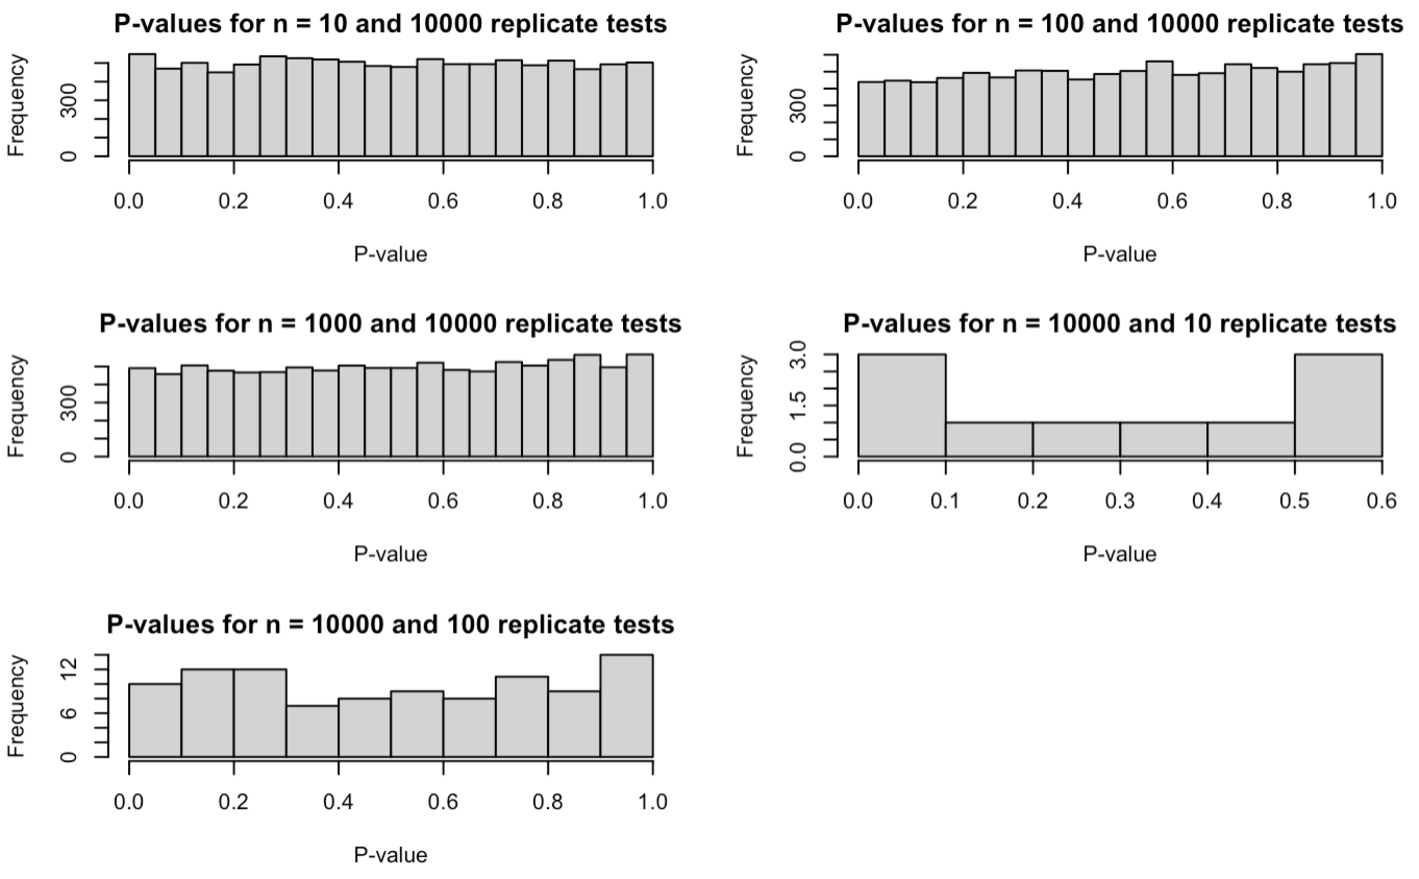
\includegraphics[width=0.8\linewidth]{Fig1}
  \caption{Histograms of impact of sample size and number of tests on P-value.}
  \label{fig:Fig1}
\end{figure}

The standard K-S test also shows misuse when the data has been rounded. For this simulation, standard normal distributions are rounded up to 4 decimal places. The histograms in Figure 2 display the distribution of P-values for the tests.

\begin{figure}[!ht]
  \centering
  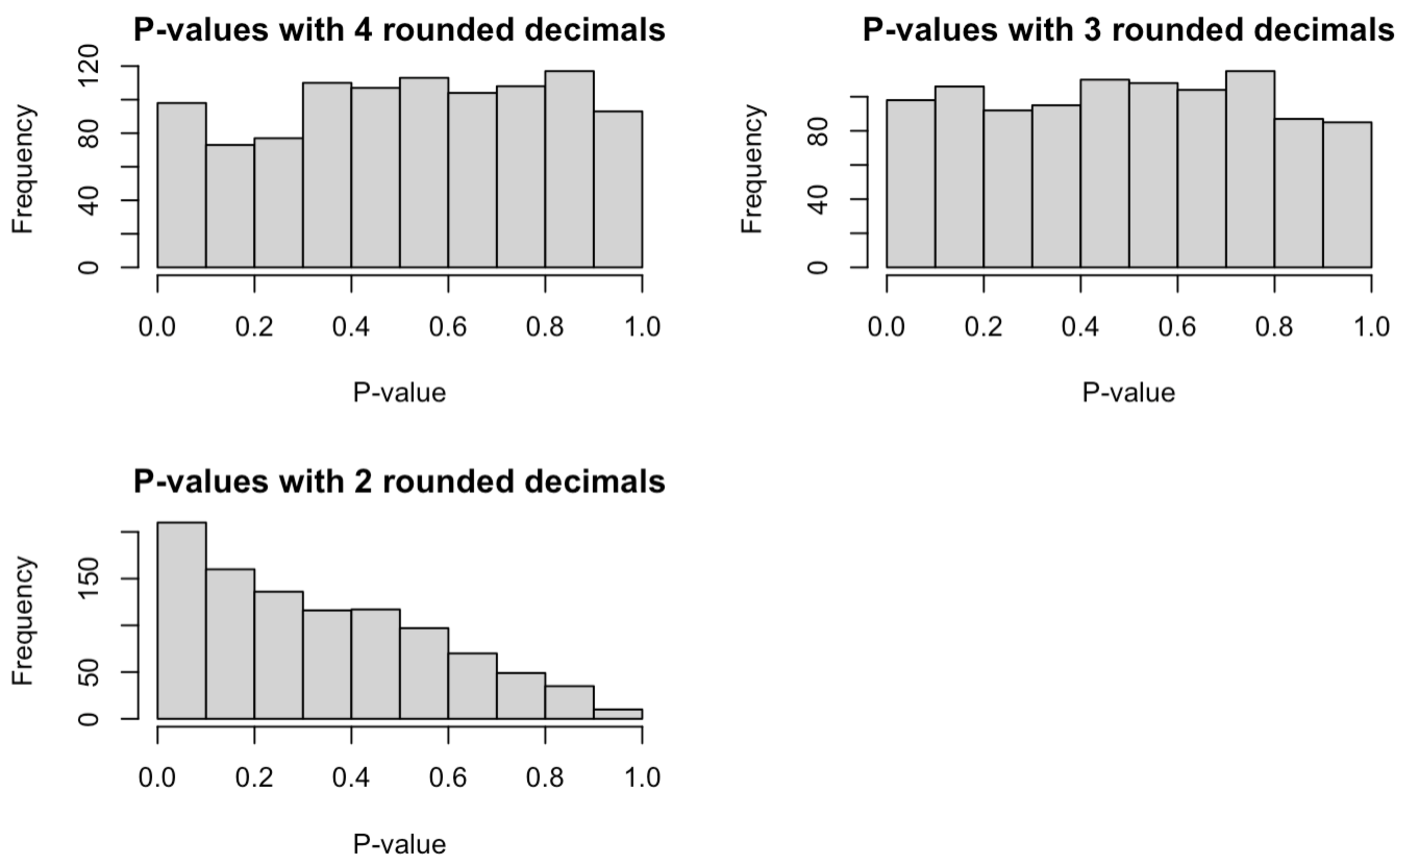
\includegraphics[width=0.8\linewidth]{Fig2}
  \caption{Histograms of P-values with rounded data}
  \label{fig:Fig2}
\end{figure}

As the level of rounding increases, the resulting P-values stray from the expected uniform distribution.

\hypertarget{sec:litrev}{%
\section{Problem Under Serial Dependence}\label{sec:litrev}}

The K-S test shows significant issues in the case of serial dependence.

\begin{table}[ht]
\centering
\begin{tabular}{rlr}
  \hline
 & Tests, Samples & PowerLevel \\ 
  \hline
1 & 10000, 10 & 0.95 \\ 
  2 & 10000, 100 & 0.96 \\ 
  3 & 10000, 1000 & 0.95 \\ 
  4 & 10, 10000 & 0.90 \\ 
  5 & 100, 10000 & 0.92 \\ 
  6 & 1000, 10000 & 0.94 \\ 
   \hline
\end{tabular}
\end{table}

\hypertarget{sec:data}{%
\section{Simulation}\label{sec:data}}

Simulation here.

\hypertarget{sec:methods}{%
\section{Real Data Analysis}\label{sec:methods}}

Real Data Analysis here.

\hypertarget{sec:disc}{%
\section{Conclusion}\label{sec:disc}}

Conclusion here.

Adding these to see the full bibliography: 

\citet{Steinskog}
\citet{Weiss}
\citet{Massey}
\citet{Lilliefors}

\bibliographystyle{chicago}
\bibliography{citations.bib}


\end{document}
